%=-=-=-=-=-=-=-=-=-=-=-=-=-=-=-=-=-=-=-=-=-=-=-=-=-=-=-=-=-=-=-=-=-=-=-=-=-=-=-=
% PREAMBLE :: sthlmNordLightDemo.tex
%=-=-=-=-=-=-=-=-=-=-=-=-=-=-=-=-=-=-=-=-=-=-=-=-=-=-=-=-=-=-=-=-=-=-=-=-=-=-=-=
%
% > > >	The following beamer class options are available
%		aspectratio=169		Change aspect ratio to 16:9
%		bibref				Include bibliography
%		sectionpages		Show section pages
%		codeminted			use minted pkg for code printing instead of listings
%							(requires additional setup & Python installed)
%		codemintedoverleaf	use minted pkg with color style support for Overleaf
% 		font sizes 			{8, 9, 10, 11, 12, 14, 17, 20} 11 Default
%
% > > > The following sthlmnord package options are available
%		mode				= dark (default)
%							= light
%=-=-=-=-=-=-=-=-=-=-=-=-=-=-=-=-=-=-=-=-=-=-=-=-=-=-=-=-=-=-=-=-=-=-=-=-=-=-=-=

\documentclass[aspectratio=169, sectionpages, codemintedoverleaf, bibref]{beamer}
% > > > Bibliography File
\newcommand{\bibfilename}{zjuref.bib}
% > > > Choose Theme
\usetheme[mode=light, language=english]{zju}
%\usetheme{sthlmnord}

% > > > Generate some Lorem Ipsum placeholder text for the demo.
\usepackage{lipsum}
\graphicspath{{./assets/}} 
% > > >	Optional use of using subfiles to make content more modular
\usepackage{subfiles}
% \usepackage{minted}

% > > > Document Information
\title{基于X的隐身系统}
\subtitle{Nord Inspired by Stockholm}
\newcommand{\titleAuthor}{Author}
\author{Jiwei Zhao}
\newcommand{\titleInstitute}{Institute}
\institute{School in Stockholm}

\newcommand{\titleMiscI}{Course}
\newcommand{\descMiscI}{Courses Title Goes Here}
\newcommand{\titleMiscII}{File}
\newcommand{\descMiscII}{\currfilebase}
\date{\today}
\titlegraphic{logo_name_v}

% > > > pdf customizations via hyperref (pkg installed by beamer)
\hypersetup{
%colorlinks=true
colorlinks=false,
linkcolor={nordNine},
citecolor={nordNine},
urlcolor={nordNine}
}

%=-=-=-=-=-=-=-=-=-=-=-=-=-=-=-=-=-=-=-=-=-=-=-=-=-=-=-=-=-=-=-=-=-=-=-=-=-=-=-=
%
%    DOCUMENT BEGINS HERE 
%
%=-=-=-=-=-=-=-=-=-=-=-=-=-=-=-=-=-=-=-=-=-=-=-=-=-=-=-=-=-=-=-=-=-=-=-=-=-=-=-=
\begin{document}

%=-=-=-=-=-=-=-=-=-=-=-=-=-=-=-=-=-=-=-=-=-=-=-=-=-=-=-=-=-=-=-=-=-=-=-=-=-=-=-=
%   TITLE START   -=-=-=-=-=-=-=-=-=-=-=-=-=-=-=-=-=-=-=-=-=-=-=-=-=-=-=-=-=-=-=
\begingroup
%   \setbeamertemplate{background canvas}{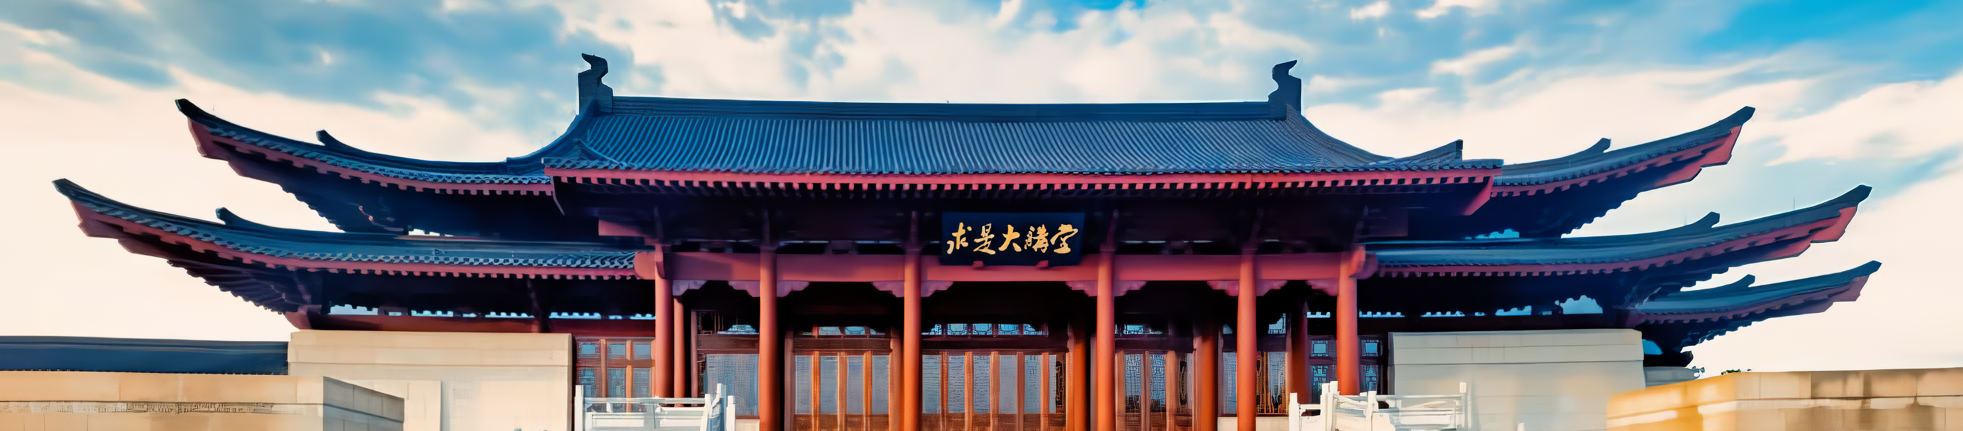
\includegraphics[width=\paperwidth,height=\paperheight]{qiushi.png}}
  \usebackgroundtemplate{\tikz[overlay,remember picture]\node[opacity=0.3]at (current page.center){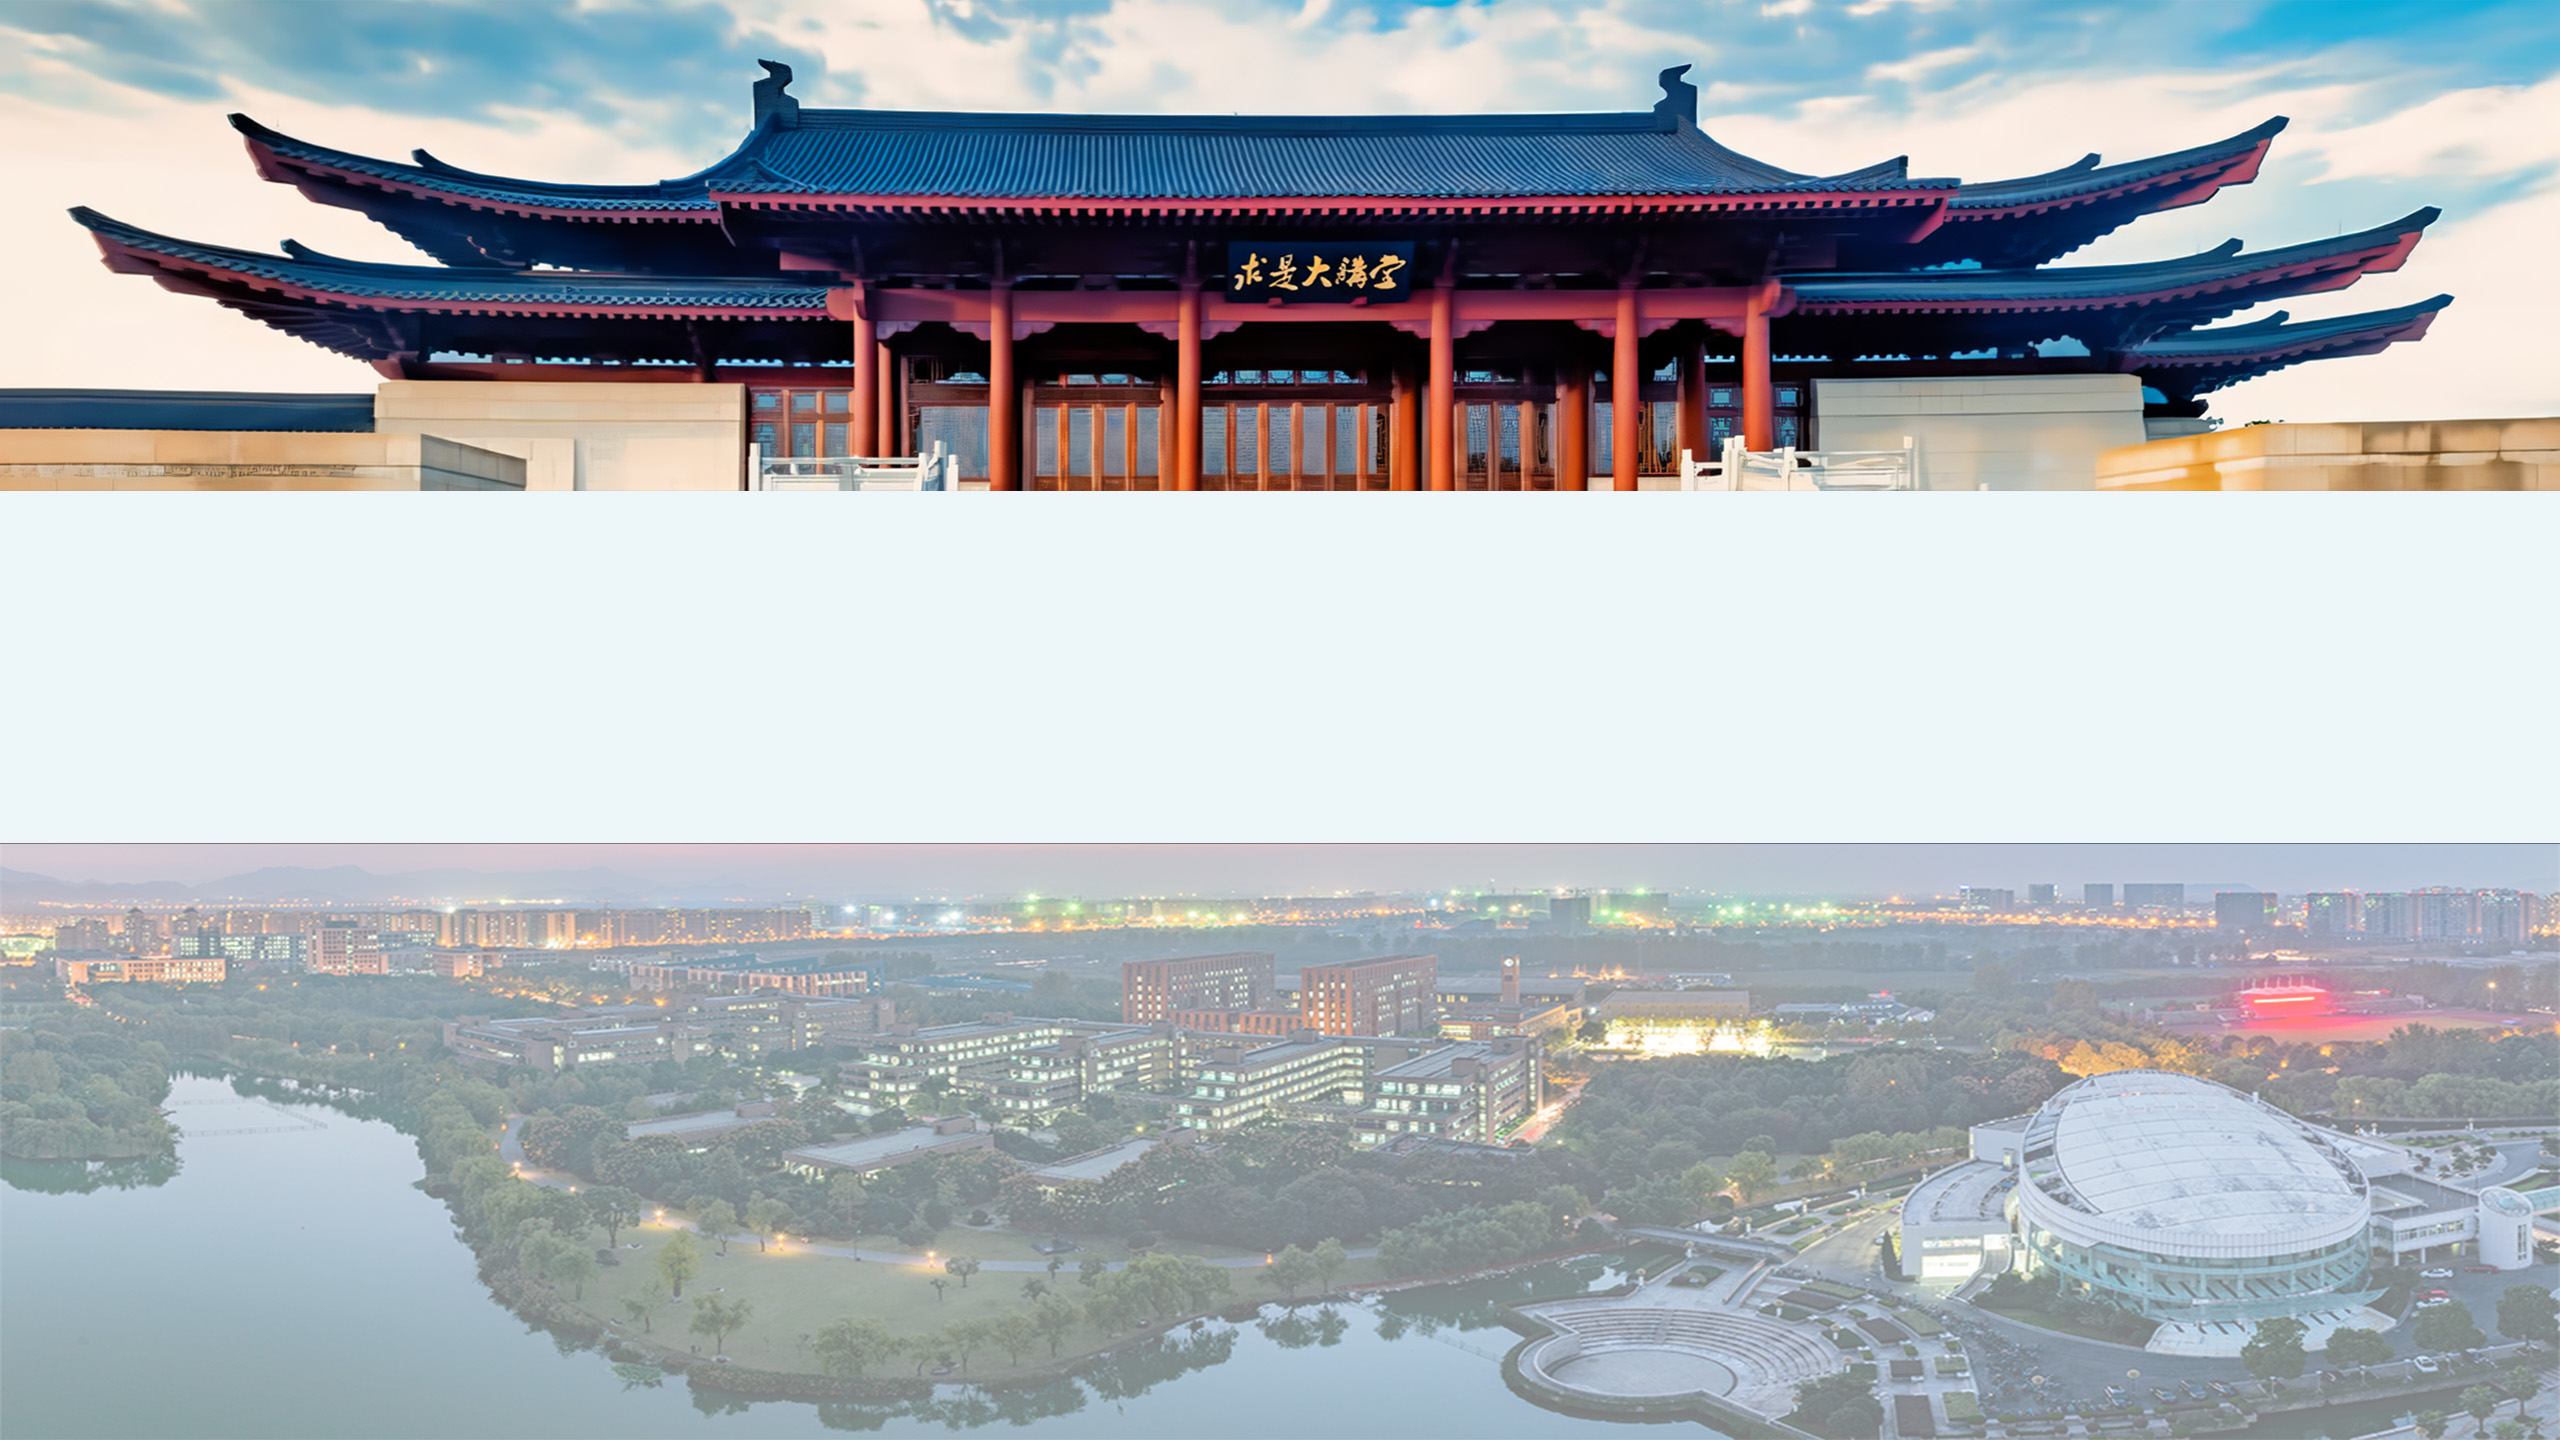
\includegraphics[width=\paperwidth]{qiushi.jpg}};}
  \titlepage
\endgroup

%   TITLE END   --==-=-=-=-=-=-=-=-=-=-=-=-=-=-=-=-=-=-=-=-=-=-=-=-=-=-=-=-=-=-=
%=-=-=-=-=-=-=-=-=-=-=-=-=-=-=-=-=-=-=-=-=-=-=-=-=-=-=-=-=-=-=-=-=-=-=-=-=-=-=-=

%=-=-=-=-=-=-=-=-=-=-=-=-=-=-=-=-=-=-=-=-=-=-=-=-=-=-=-=-=-=-=-=-=-=-=-=-=-=-=-=
%   TABLE OF CONTENTS START   -=-=-=-=-=-=-=-=-=-=-=-=-=-=-=-=-=-=-=-=-=-=-=-=-=
\begin{frame}[allowframebreaks]%
    \transfade%淡入淡出效果
	\vspace{-0.56cm}
    \addtocontents{toc}{\protect\thispagestyle{empty}}
    \pagenumbering{gobble}
		\frametitle{Table of contents}%
		\textbf{\tableofcontents[hideallsubsections]}
    \addtocounter{framenumber}{-1}  %目录页不计算页码
    \pagenumbering{}
\end{frame}

%   TABLE OF CONTENTS END   -=-=-=-=-=-=-=-=-=-=-=-=-=-=-=-=-=-=-=-=-=-=-=-=-=-=
%=-=-=-=-=-=-=-=-=-=-=-=-=-=-=-=-=-=-=-=-=-=-=-=-=-=-=-=-=-=-=-=-=-=-=-=-=-=-=-=

%=-=-=-=-=-=-=-=-=-=-=-=-=-=-=-=-=-=-=-=-=-=-=-=-=-=-=-=-=-=-=-=-=-=-=-=-=-=-=-=
% SECTION 
%=-=-=-=-=-=-=-=-=-=-=-=-=-=-=-=-=-=-=-=-=-=-=-=-=-=-=-=-=-=-=-=-=-=-=-=-=-=-=-=
\section{Background Information}
\subsection{sdsd}
\subfile{0-slides/tex.slide.useMetroWarning}
\subfile{0-slides/tex.slide.majorFeatures}
\subfile{0-slides/tex.slide.history}
\subsection{sdsd}
\subfile{0-slides/tex.slide.noGuarantee}
\subfile{0-slides/tex.slide.availableGitHub}
\subfile{0-slides/tex.slide.availableOverleaf}
\subfile{0-slides/tex.slide.ctanPackages}
\subfile{0-slides/tex.slide.customPackages}

%=-=-=-=-=-=-=-=-=-=-=-=-=-=-=-=-=-=-=-=-=-=-=-=-=-=-=-=-=-=-=-=-=-=-=-=-=-=-=-=
% SECTION 
%=-=-=-=-=-=-=-=-=-=-=-=-=-=-=-=-=-=-=-=-=-=-=-=-=-=-=-=-=-=-=-=-=-=-=-=-=-=-=-=
\section{Colors}

\subfile{0-slides/tex.slide.nordPaletteLight}
\subfile{0-slides/tex.slide.nordPaletteTextLight}
\subfile{0-slides/tex.slide.nordPaletteTextHighlightLight}

%=-=-=-=-=-=-=-=-=-=-=-=-=-=-=-=-=-=-=-=-=-=-=-=-=-=-=-=-=-=-=-=-=-=-=-=-=-=-=-=
% SECTION 
%=-=-=-=-=-=-=-=-=-=-=-=-=-=-=-=-=-=-=-=-=-=-=-=-=-=-=-=-=-=-=-=-=-=-=-=-=-=-=-=
\section{Deck Structures}

\subfile{0-slides/tex.slide.blocks}
\subfile{0-slides/tex.slide.listsEnumerate}
\subfile{0-slides/tex.slide.listsItemize}
\subfile{0-slides/tex.slide.listsDescription}
\subfile{0-slides/tex.slide.codeblocks}

\subfile{0-slides/tex.slide.exampleSlide}
\subfile{0-slides/tex.slide.theoremSlide}

%=-=-=-=-=-=-=-=-=-=-=-=-=-=-=-=-=-=-=-=-=-=-=-=-=-=-=-=-=-=-=-=-=-=-=-=-=-=-=-=
% SECTION 
%=-=-=-=-=-=-=-=-=-=-=-=-=-=-=-=-=-=-=-=-=-=-=-=-=-=-=-=-=-=-=-=-=-=-=-=-=-=-=-=
\section{Fonts}

\subfile{0-slides/tex.slide.fonts}

%=-=-=-=-=-=-=-=-=-=-=-=-=-=-=-=-=-=-=-=-=-=-=-=-=-=-=-=-=-=-=-=-=-=-=-=-=-=-=-=
% SECTION 
%=-=-=-=-=-=-=-=-=-=-=-=-=-=-=-=-=-=-=-=-=-=-=-=-=-=-=-=-=-=-=-=-=-=-=-=-=-=-=-=
\section{Mathematics}

\subfile{0-slides/tex.slide.typeMathematics}
\subfile{0-slides/tex.slide.tikz}
\subfile{0-slides/tex.slide.mathExampleExpand}

\subfile{0-slides/tex.slide.mathExampleCTS}
\subfile{0-slides/tex.slide.mathExampleDiceCoins.tex}
\subfile{0-slides/tex.slide.mathSets}

%=-=-=-=-=-=-=-=-=-=-=-=-=-=-=-=-=-=-=-=-=-=-=-=-=-=-=-=-=-=-=-=-=-=-=-=-=-=-=-=
% SECTION 
%=-=-=-=-=-=-=-=-=-=-=-=-=-=-=-=-=-=-=-=-=-=-=-=-=-=-=-=-=-=-=-=-=-=-=-=-=-=-=-=
\section{References}

\begin{frame}[allowframebreaks]{References}
	\printbibliography[title={References}]%
\end{frame}

% 谢辞部分
{	
	% \pagenumbering{gobble}
	\nologo
	\usebackgroundtemplate{\tikz[overlay,remember picture]\node[opacity=0.3]at (current page.center){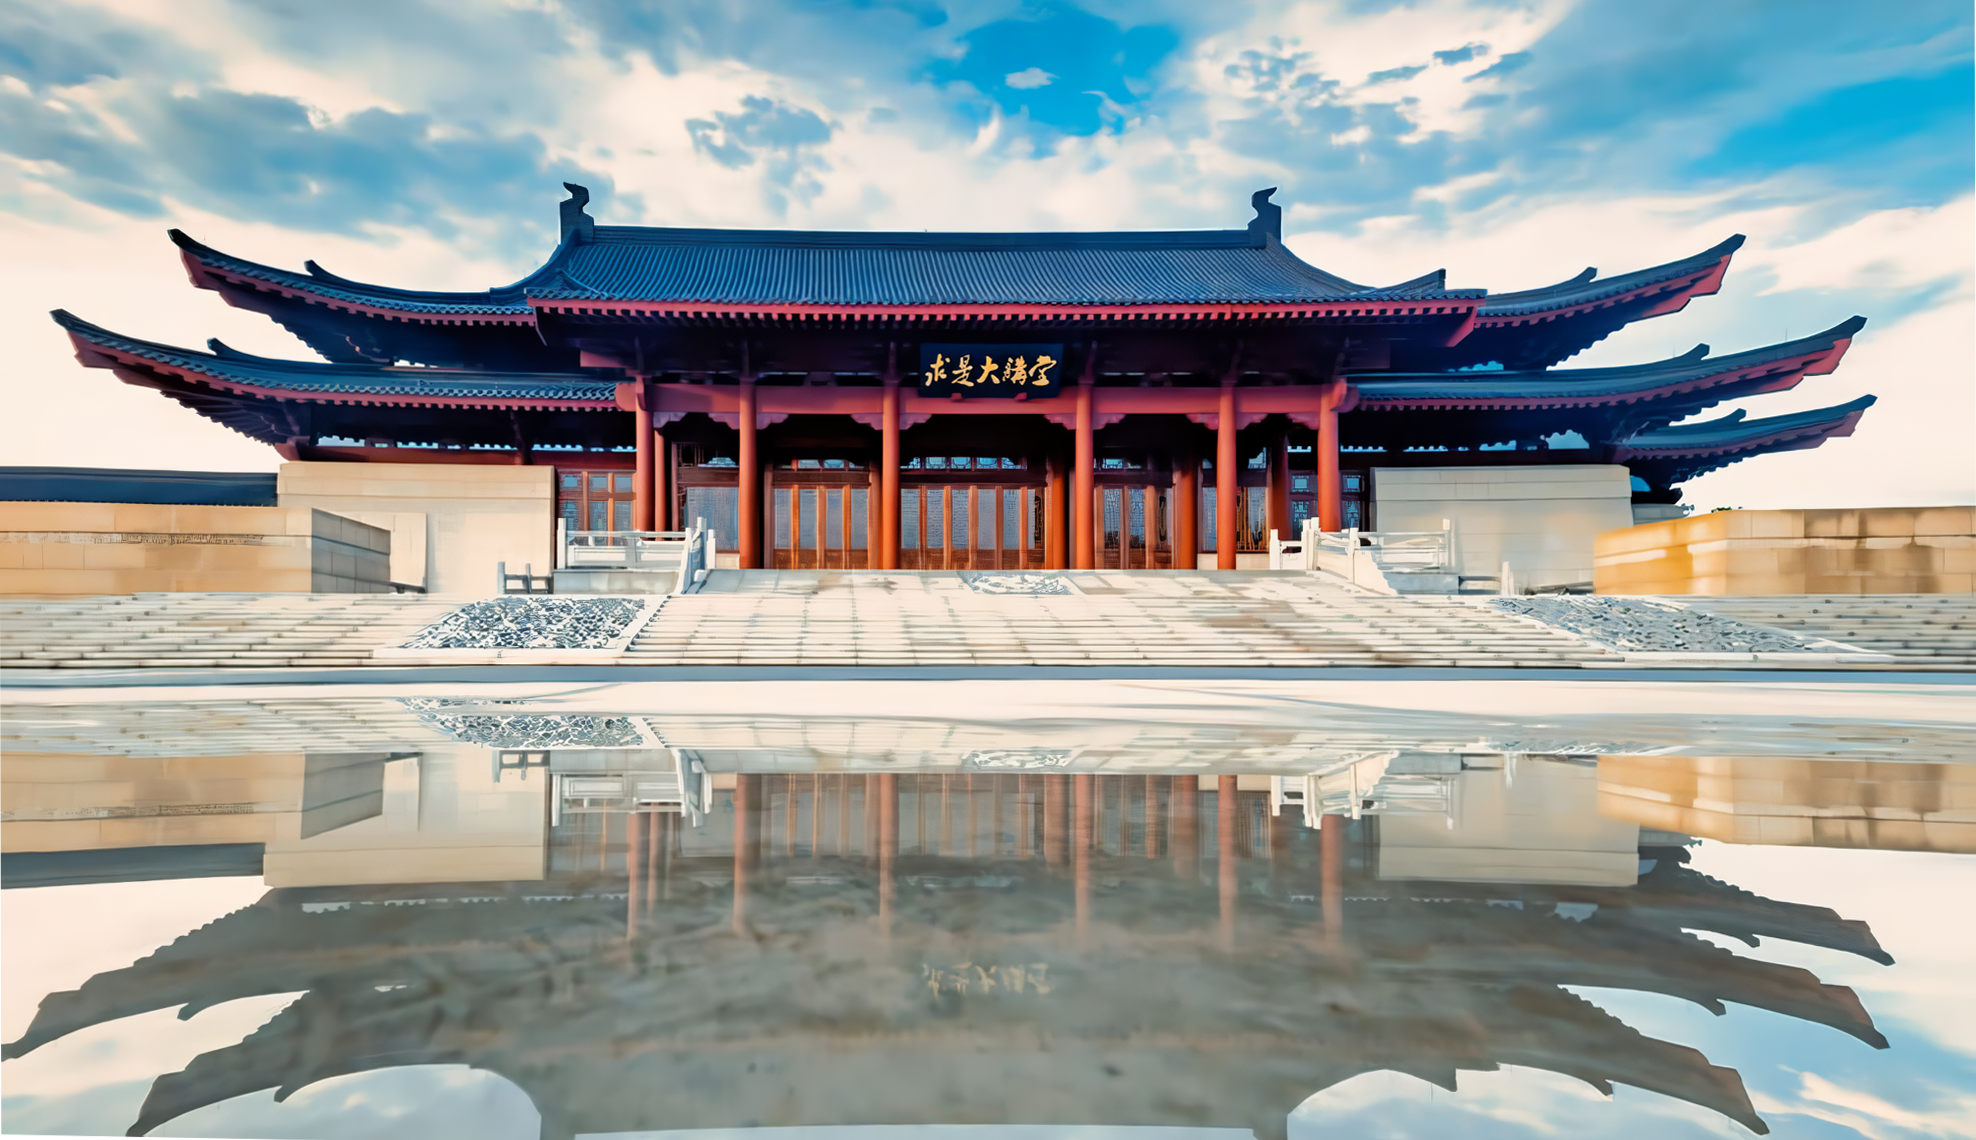
\includegraphics[width=\paperwidth]{qiushi2.png}};}
	\begin{frame}[allowframebreaks]
		\vspace{13ex}
		\textcolor{nordEleven}{\textbf{\Huge{\centerline{Thank you !}}}}
	\end{frame}
	\addtocounter{framenumber}{-1}  %目录页不计算页码
    \pagenumbering{}
}

\end{document}
%=+=+=+=+=+=+=+=+=+=+=+=+=+=+=+=+=+=+=+=+=+=+=+=+=+=+=+=+=+=+=+=+=+=+=+=+=+=+=+=
% END OF FILE
%=+=+=+=+=+=+=+=+=+=+=+=+=+=+=+=+=+=+=+=+=+=+=+=+=+=+=+=+=+=+=+=+=+=+=+=+=+=+=+=
